
\section{Elektromagnetische Felder}
	\subsection{Elektromagnetische Wellenausbreitung}
		
		\begin{minipage}{4.3cm}
			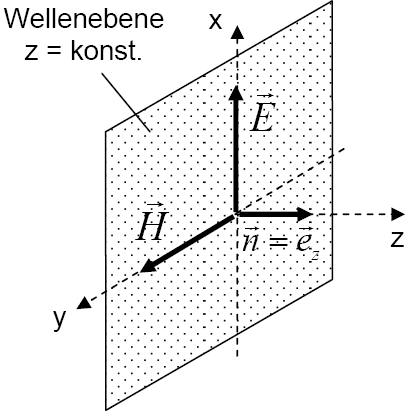
\includegraphics[width=4cm]{./bilder/EMW_EbeneWelle.png} 
        \end{minipage}
		\renewcommand{\arraystretch}{1.6}
		\begin{tabular}{| c | c | c | }
			\hline
				\multicolumn{3}{| c |}{\textbf{Definition Ebenen}}    \\
			\hline
				\multicolumn{3}{| l |}{\textbf{Wellenebene: } Durch $\vec{H}$ und $\vec{E}$ aufgespannt.} \\
				\multicolumn{3}{| l |}{\textbf{Trennebene: } Grenzfläche zwischen den beiden Medien.} \\ 
				\multicolumn{3}{| l |}{\textbf{Einfallsebene: } Durch Richtungsvektor der Wellenausbreitung
				und $\vec{n}_{Trennebene}$ aufgespannt.} \\
			\hline
    		\hline
				\textbf{Wellenwiderstand} & \textbf{Wellenwid.} - Vakuum & \textbf{Wellengeschwindigkeit,
				-konstante}\\
			\hline
				$Z=\dfrac{E}{H}=\sqrt{\frac{\mu}{\varepsilon}}$ 
				& $Z_0 = \sqrt{\frac{\mu_0}{\varepsilon_0}} = 120\pi \Omega$
				& $v=\frac{1}{\sqrt{\mu \varepsilon}} \quad v_0 = c\approx 3*10^8 \frac{m}{s}; \qquad \beta =
				\omega \sqrt{\mu \epsilon}$
				\\
			\hline
				\textbf{Orientierung} & \textbf{Poynting Vektor} & \textbf{Konstanten} \\
			\hline
				$Z \cdot \vec{H} = \vec{n} \times \vec{E}$
				& $\vec{S}=\vec{E}\times\vec{H}$
				& $\varepsilon_0=8,854\cdot 10^{-12}[\frac{As}{Vm}] \quad
				\mu_0=4\pi\cdot 10^{-7}[\frac{Vs}{Am}]$ \\
			\hline
			\hline
				\multicolumn{3}{| c |}{\textbf{Gebräuchliche Indizes}} \\
			\hline	
				\textbf{i}: incident = einfallend
				& \textbf{r}: reflected = reflektiert
				& \textbf{t}: transmitted = übermittelt 	\\
			\hline
   		\end{tabular}
		\renewcommand{\arraystretch}{1}


		
	\subsubsection{Leitender Halbraum}	
		Die Welle wird an der Trennebene vollständig reflektiert. \\
				
		\begin{minipage}{4cm}
			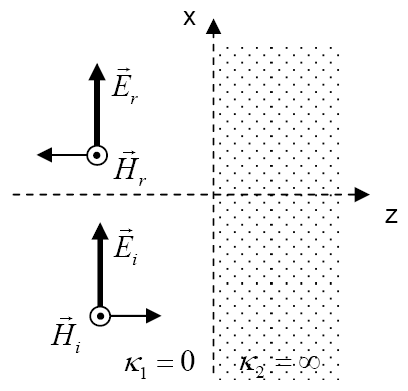
\includegraphics[width=3.8cm]{./bilder/EMW_LHR_SenkrechtEinfallendeWelle.png} 
        \end{minipage}
		\renewcommand{\arraystretch}{1.6}
		\begin{tabular}{| l  | l |}
			\hline
				\multicolumn{2}{|l|}{\textbf{Senkrecht einfallende Ebene Welle}} \\		
				\hline
				$E_r + E_i = 0 \Rightarrow E_r = - E_i$ & \\
				$\vec{E}_i (z) = \vec{e}_x E_i e^{-j \beta_1 z} \qquad  \qquad 
				\vec{E}_r (z) = \vec{e}_x E_r e^{+j \beta_1 z}$
				
				& $\vec{H}_i (z) = \vec{e}_y \frac{E_i}{Z_1} e^{-j \beta_1 z} \qquad  \qquad 
				\vec{H}_r (z) = \vec{e}_y \frac{E_i}{Z_1} e^{+j \beta_1 z}$
				\\
				
				$\vec{E}_1 (z) = \vec{e}_x E_i (e^{-j \beta_1 z} - e^{+ j \beta_1 z}) = 
				-\vec{e}_x j 2 E_i \sin{(\beta_1 z)}	$
				& 
				$\vec{H}_1 (z) = \vec{e}_y \frac{E_i}{Z_1} (e^{-j \beta_1 z} + e^{+ j \beta_1 z}) = 
				\vec{e}_y j 2 \frac{E_i}{Z_1} \cos{(\beta_1 z)}	$ \\
				
				$E_1 (z,t) = \text{Re}\left\{ \vec{E}_1(z) e^{j \omega t}\right\} =
				\vec{e}_x 2 E_i \sin{(\beta_1 z)} \sin{(\omega t)}	$
				& 
				$H_1 (z,t) = \text{Re}\left\{ \vec{H}_1(z) e^{j \omega t}\right\} =
				\vec{e}_y 2 \frac{E_i}{Z_1} \cos{(\beta_1 z)} \cos{(\omega t)}	$\\		
				
			\hline
   		\end{tabular}
		\renewcommand{\arraystretch}{1}	
		
		\begin{minipage}{4.3cm}
			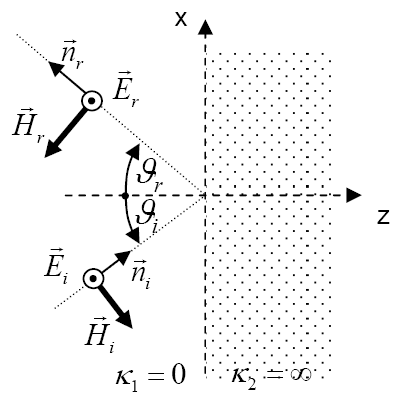
\includegraphics[width=4cm]{./bilder/EMW_LHR_SchraegSenkrechtPolarisiert.png} 
        \end{minipage}
		\renewcommand{\arraystretch}{1.6}
		\begin{tabular}{| c || c | }
			\hline
				\multicolumn{2}{|c|}{\textbf{Schräg einfallende Welle}} \\
			\hline
				\textbf{Senkrechte Polarisation}
				& 
				\textbf{Parallele Polarisation} \\	
			\hline		
				$\vec{E} \perp $ Einfallsebene
				& 
				$\vec{E} \parallel $ Einfallsebene \\
			\hline	
 				$\vec{n}_i = \vec{e}_x \sin(\vartheta_i)+\vec{e}_z \cos(\vartheta_i)$&\\
 				$\vec{n}_r=\vec{e}_x \sin(\vartheta_i)- \vec{e}_z \cos(\vartheta_i)$ &\\
  				$\vec{r}=\vec{e}_x x+\vec{e}_z z;$ 
 				$E_r=-E_i; \vartheta_r =\vartheta_i$&\\
 				$\vec{E}_{i(x,z)} =\vec{e}_y E_i e^{-j \beta_1 \vec{n}_i \vec{r}}$&\\ 
 				$\vec{E}_r(x,z) =\vec{e}_y E_i e^{-j \beta_1 \vec{n}_r
 				\vec{r}}=- \vec{e}_y E_i e^{-j \beta_1
 				(x\sin(\vartheta_i)-z\cos(\vartheta_i))}$&\\
 				$\vec{H}_{r(x,z)}=\frac{1}{z_1}(\vec{n}_r\times \vec{E}_{r(x,z)})$&\\
 				\hline
 				\multicolumn{2}{|l|}{
				$\vec{n_i}=
				\frac{\beta_x}{\beta}\vec{e}_x + \frac{\beta_y}{\beta} \vec{e}_y + 
				\frac{\beta_z}{\beta} \vec{e}_z
				\qquad \qquad \beta=\sqrt{\beta_x^2+\beta_y^2+\beta_z^2}$}\\
			\hline
   		\end{tabular}
		\renewcommand{\arraystretch}{1}	
		\begin{minipage}{4.3cm}
			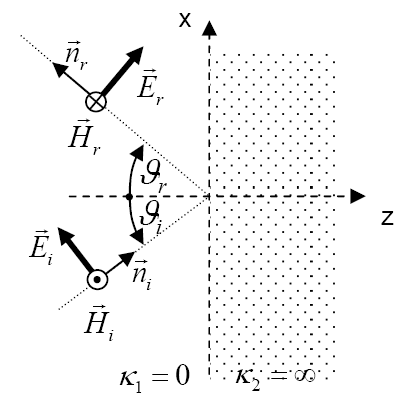
\includegraphics[width=4cm]{./bilder/EMW_LHR_SchraegParallelPolarisiert.png} 
        \end{minipage}	

	\subsubsection{Dielektrischer Halbraum}
		Je nach Einfallswinkel $\vartheta_i$ wird die Welle nicht nur reflektiert, sondern dringt in das
		zweite Medium ein. \\
		
		\renewcommand{\arraystretch}{1.6}
		\begin{tabular}{| l  | l | l |}
			\hline
				\textbf{Transmissionskoeffizient} & \textbf{Reflexionskoeffizient} &
				\textbf{Stehwellenverhältnis}
				\\
			\hline
				$t = \dfrac{E_t}{E_i} = \dfrac{2 Z_2}{Z_2 + Z_1} \qquad 1 + r = t$ 
				& $r = \dfrac{E_r}{E_i} = \dfrac{Z_2 - Z_1}{Z_2 + Z_1} \qquad  |r| = \dfrac{SWR - 1}{SWR + 1}$
				& $SWR = \dfrac{|E|_{max}}{|E|_{min}} = \dfrac{1 + |r|}{1 - |r|}$ \\
			\hline
   		\end{tabular}
		\renewcommand{\arraystretch}{1}	
		
		\begin{minipage}{4cm}
			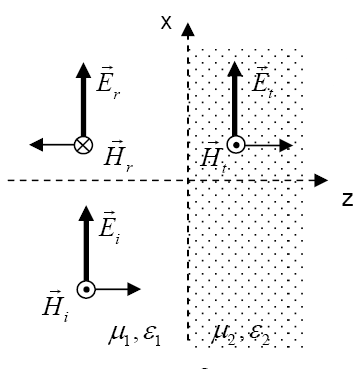
\includegraphics[width=4cm]{./bilder/EMW_DHR_SenkrechtEinfallendeWelle.png} 
        \end{minipage}
		\renewcommand{\arraystretch}{1.6}
		\begin{tabular}{| l  | l |}
			\hline
				\multicolumn{2}{|c|}{\textbf{Senkrecht einfallende Ebene Welle}} \\
			\hline
				$E_i + E_r = E_t$ &
				$H_i + H_r = H_t$ \\
			\hline
   		\end{tabular}
		\renewcommand{\arraystretch}{1}	
		
				
		
		
		\begin{minipage}{4.3cm}
			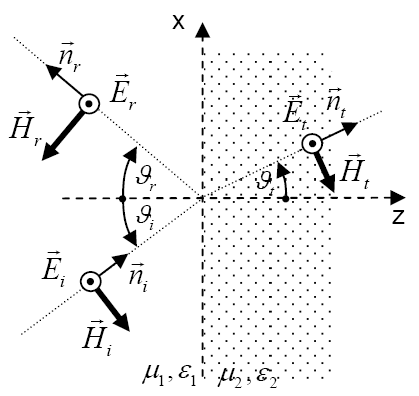
\includegraphics[width=4cm]{./bilder/EMW_DHR_SchraegSenkrechtPolarisiert.png} 
        \end{minipage}
		\renewcommand{\arraystretch}{1.6}
		\begin{tabular}{| c || c | }
			\hline
				\multicolumn{2}{|c|}{\textbf{Schräg einfallende Welle}} \\
			\hline
				\multicolumn{2}{|c|}{$\dfrac{\sin{\vartheta_t}}{\sin{\vartheta_i}} = \sqrt{\dfrac{\mu_1
				\epsilon_1}{\mu_2 \epsilon_2}} \qquad \vartheta_r = \vartheta_i$} \\
			\hline
				\textbf{Senkrechte Polarisation}
				& 
				\textbf{Parallele Polarisation} \\	
			\hline		
				$ \sin^2 \vartheta_{Brewster_1} = \dfrac{1 - \frac{\mu_1 \epsilon_2}{\mu_2 \epsilon_1}}{1 -
				\left(\frac{\mu_1}{\mu_2}\right)^2}$ 
				& $ \sin^2 \vartheta_{Brewster_2} = \dfrac{1 - \frac{\mu_2 \epsilon_1}{\mu_1 \epsilon_2}}{1 -
				\left(\frac{\epsilon_1}{\epsilon_2}\right)^2}$ \\
				$r_{SP} = \dfrac{E_r}{E_i} = \dfrac{Z_2 \cos{\vartheta_i} - Z_1 \cos{\vartheta_t}}{Z_2
				\cos{\vartheta_i} + Z_1 \cos{\vartheta_t}}$
				& $r_{PP} = \dfrac{E_r}{E_i} = \dfrac{Z_2 \cos{\vartheta_t} - Z_1 \cos{\vartheta_i}}{Z_2
				\cos{\vartheta_t} + Z_1 \cos{\vartheta_i}}$ \\
				$t_{SP} =  \dfrac{E_t}{E_i} = \dfrac{2 Z_2 \cos{\vartheta_i}}{Z_2 \cos{\vartheta_i} + Z_1
				\cos{\vartheta_t}}$
				& $t_{PP} = \dfrac{E_t}{E_i} =  \dfrac{2 Z_2 \cos{\vartheta_t}}{Z_2 \cos{\vartheta_t} + Z_1
				\cos{\vartheta_i}}$ \\
			\hline
   		\end{tabular}
		\renewcommand{\arraystretch}{1}	
		\begin{minipage}{4.3cm}
			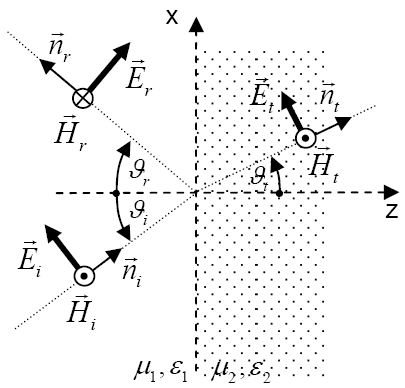
\includegraphics[width=4cm]{./bilder/EMW_DHR_SchraegParallelPolarisiert.png} 
        \end{minipage}	
		
	\subsection{Hertz'scher Dipol}		
		\begin{minipage}{4.8cm}
			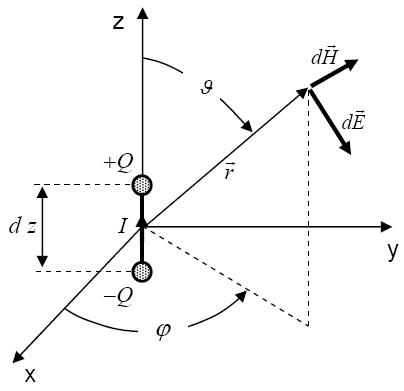
\includegraphics[height=4.7cm]{./bilder/LinAnt_HerzscherDipol.png}
        \end{minipage}
		\renewcommand{\arraystretch}{1.6}
		\begin{tabular}{| c | c | c | c |}
    		\hline
    	\multicolumn{2}{| c |}{\textbf{Magnetische Feld}} & \multicolumn{2}{| c
    	|}{\textbf{Wellenwiderstand}} \\
    		\hline
    	\multicolumn{2}{| c |}{$\vec{H} = \vec{e}_{\varphi} \dfrac{j \beta \sin \vartheta}{4 \pi r}
    	e^{-j \beta r} \int\limits_{-l}^{+l}I(z) e^{j \beta z \cos \vartheta} dz$}
    	& \multicolumn{2}{| c |}{$Z_0 = \dfrac{dE}{dH} \sqrt{\dfrac{\mu_0}{\epsilon_0}}$}
    	\\
			\hline
    	\multicolumn{4}{| c |}{\textbf{Fernfeld} - ($\beta z = 2 \pi z / \lambda \ll 1$)} \\        
    		\hline
    	\multicolumn{2}{| c |}{$\vec{H} = \vec{e}_{\varphi} \dfrac{I_0 l \sin \vartheta}{4 \pi r} j
    	\beta e^{-j \beta r} $} 
    	& \multicolumn{2}{| c |}{$\vec{E} = \vec{e}_{\vartheta} Z_0 \dfrac{I_0 l \sin \vartheta}{4
    	\pi r} j \beta e^{-j \beta r} $}\\
			\hline
    		\hline   
    	\multicolumn{2}{| c |}{\textbf{Strahlungsleistung}} & \textbf{Strahlungswid.} &
    	\textbf{Strahlungschar.} \small{($\Phi_0 = \Phi(\frac\pi2)$)}  \\
    		\hline
    	\multicolumn{2}{| c |}{$\bar{P}_s = \dfrac{2 \pi}{3} Z_0 \left( \dfrac{l}{\lambda}\right)^2
    	I_0^2 = 
    	\dfrac{1}{2}
    	\text{Re} \left\{ \oiint\limits_{F \infty} (\vec{E}
    	\times
    	\vec{H}^* ) d \vec{F} \right\}  $}
    	& $R_s=\frac{2\pi}{3}Z_0 \left(\frac{l}{\lambda}\right)^2$
    	& $\Phi(\vartheta) = \dfrac{Z_0}{4} \left( \dfrac{l}{\lambda} \right)^2 I_0^2
    	\sin^2\vartheta$
    	\\
		\hline
   		\end{tabular}
		\renewcommand{\arraystretch}{1}
	
		
	\subsection{Lineare Antennen}
		\begin{minipage}{2.2cm}
			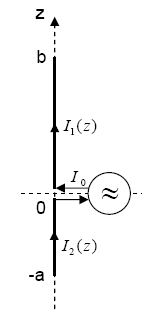
\includegraphics[height=4.5cm]{./bilder/LinAnt_Stromverteilung.png}
        \end{minipage}
		\begin{minipage}{12.7cm}
		\renewcommand{\arraystretch}{1.6}
		\begin{tabular}{| c | c |}
    		\hline
    	\multicolumn{2}{| c |}{\textbf{Strahlung linearer Antennen} - siehe Bild rechts} \\        
    		\hline
    $\vec{H}(\vec{r}_P) = - \frac{j}{2 \lambda r_p} e^{-j 2 \pi \frac{r_p}{\lambda}}     
    \int\limits_A^B I(\vec{r}_Q) e^{j 2 \pi \frac{\vec{n} \vec{r}_Q}{\lambda}} (\vec{n} \times
    d \vec{r}_Q) $
	&
    $ \vec{E}(\vec{r}_p) = - Z_0 \left[ \vec{n} \times \vec{H} (\vec{r}_p) \right] $
    \\
			\hline
    		\hline   
    	\multicolumn{2}{| c |}{\textbf{Strahlungscharakteristik}}
    	\\
    		\hline
    \multicolumn{2}{| c |}{$ \Phi(\vec{n}) = \dfrac12 Z_0 r_P^2 \vec{H} (\vec{r}_p) \cdot \vec{H}^*
    (\vec{r}_p) = \vec{n} r^2_p \bar{S}(\vec{r}_p) = \dfrac{1}{2} \vec{n} r_p^2 \text{Re} \left\{
    -Z_0 ( \vec{n} \times \vec{H} ) \times \vec{H}^* \right\} $} \\
			\hline
    		\hline
    	\multicolumn{2}{| c |}{\textbf{Stromverteilung auf linearen Antennen} - siehe Bild links} \\
    		\hline
    	$ I_1 (z) = \dfrac{\sin{[\beta (b - z)]}}{\sin{[\beta b]}} I_0 ; \quad 0 \leq z \leq
    	b$
    	& 
    	$ I_2 (z) = \dfrac{\sin{[\beta (a + z)]}}{\sin{[\beta a]}} I_0 ; \quad -a \leq z \leq
    	0$ \\
    	
    		\hline
    		\hline
    	\textbf{Strahlungsleistung} & \textbf{Strahlungswiderstand} \\
    		\hline
    	$ \bar{P}_S = \int\limits_0^{2\pi}\int\limits_0^{\pi} \Phi(\vartheta) \sin \vartheta \cdot
    	d \vartheta \cdot d \varphi	$ 
    	& 
    	$ R_S = \dfrac{2}{I_0^2 } \int\limits_0^{2\pi}\int\limits_0^{\pi} \Phi(\vartheta) \sin \vartheta \cdot
    	d \vartheta \cdot d \varphi	$ \\
    		\hline
   		\end{tabular}
		\renewcommand{\arraystretch}{1}
        \end{minipage}		
		\begin{minipage}{4.5cm}
			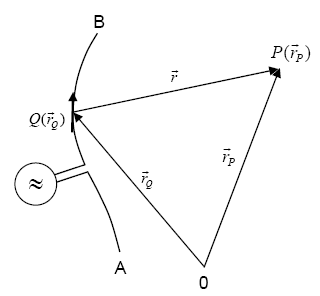
\includegraphics[height=4cm]{./bilder/LinAnt_Strahlung.png}
        \end{minipage}
		
	\subsubsection{Richtcharakteristika}
	\begin{center}
		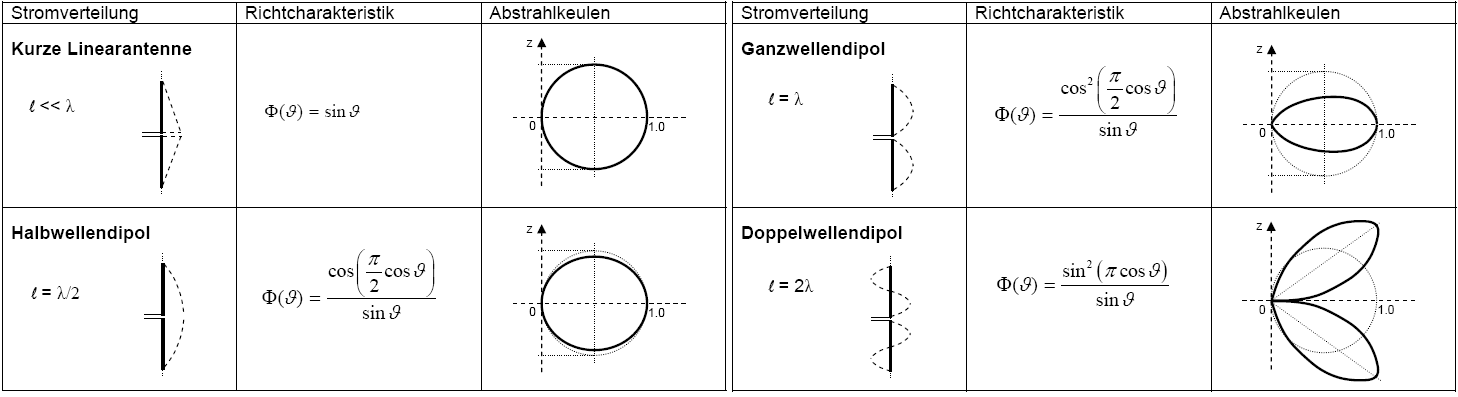
\includegraphics[width=19cm]{./bilder/LinAnt_Richtcharakteristika.png}    
  \end{center}

  \section{Integral-Gesetze der Elektrotechnik}
	\renewcommand{\arraystretch}{2}
	\begin{tabular}{|p{2.5cm}||p{2.7cm}|p{4cm}|p{2.7cm}|p{5cm}|}
	\hline
	& \textbf{Elektr. Feld} & \textbf{Magn. Feld} & \textbf{Strömungsfeld} & \textbf{Bemerkung}\\
	\hline \hline
	Feldgrösse & $\vec{E}$, $\vec{D}$ & $\vec{H}$, $\vec{B}$
	& $\vec{E}$, $\vec{J}$ &\\
	\hline
	Konstante
		& \parbox{2.7cm}{$\varepsilon_0 = 8.854 \cdot 10^{-12}$\\
		{\tiny Dielektrizitätskonstante} \vspace{.1cm}} 
		& \parbox{4cm}{$\mu_0 = 4 \pi \, 10^{-7}$\\ {\tiny Permeabilitätskonstante} \vspace{.1cm}} 
		& \parbox{2.7cm}{$\sigma=\frac{1}{\rho}$ \\ {\tiny Spezifische
		Leitfähigkeit}\vspace{.1cm}} &\\ 
	\hline
	Stoffgleichung & $\vec{D}=\varepsilon_0\varepsilon_r\vec{E}$ & $\vec{B}=\mu_0\mu_r\vec{H}$
	& $\vec{J}=\sigma\vec{E}$ &
	\\
	\hline
	Kraft & $\vec{F_C}=q\vec{E}$ & $\vec{F_L}=q(\vec{v}\times\vec{B})$ &&\\
	\hline
	\parbox{2.5cm}{Fluss\\{\tiny (durch Fläche A)}} & $\Psi_{el}=\int\vec{D}\vec{dA}$ &
	$\Phi_m=\int\vec{B}\vec{dA}$ \textsuperscript{1)}&
	$I=\int\vec{J}\vec{dA}$ & \textsuperscript{1)} bei Spulen:
	$\Psi_m=\sum_i\Phi_i\approx N \Phi$\\
	\hline
	\parbox{2.5cm}{Spannung \\{\tiny (Weg A$\to$B)}} & $U_{AB}=\int\limits_{A}^B
	\vec{E}\vec{ds}$ & $V_{m_{AB}}=\int\limits_{A}^B\vec{H}\vec{ds}$ 
	& $U_{AB}=\int\limits_{A}^B\vec{E}\vec{ds}$ & \\
	\hline
	Schaltelemente & $Q=CU$ & $\Psi_m=LI$, $\Psi_{m21}=M_{21}I_1$
	& $I=GU$, $U=RI$ & $R_m=\frac{1}{\Lambda}$, $R=\frac{1}{G}$\\
	\hline
	\parbox{2.5cm}{Hüllengesetz \\ {\tiny (Quellengleichungen)}}
		& \parbox{2.7cm}{
			\vspace{.1cm}$\oint\vec{D}\vec{dA}=\sum Q_i$ \vspace{.1cm}
			Maxwell IV
			\vspace{.1cm}}
		& \parbox{4cm}{
			\vspace{.1cm}$\oint\vec{B}\vec{dA}=0$
			\textsuperscript{2)} \\
			Maxwell III
			\vspace{.1cm}} 
		& \parbox{2.7cm}{
			$\oint\vec{J}\vec{dA}=0$\\
			Kirchhoff 1}
		& \parbox{5cm}{\textsuperscript{2)} ohne Verschiebungsstrom (käme ggf. noch
		dazu)} \\
	\hline
	Umlaufspannung 
		& \parbox{2.7cm}{
			\vspace{.1cm}
			$\oint\vec{E}\vec{ds}=0-\dot{\Phi}_m$ \\ 
			{\tiny Induktionsgesetz}\\Maxwell II
			\vspace{.1cm}}
		& \parbox{4cm}{
			\vspace{.1cm}
			$\oint\vec{H}\vec{ds}=\theta+\dot{\Psi}_{el}$ \\ 
			{\tiny Vollständiges Durchflutungsgesetz} \\Maxwell I
			\vspace{.1cm}}
		& \parbox{2.7cm}{
			\vspace{.1cm}
			$\oint\vec{E}\vec{ds}=0-\dot{\Phi}$ \\ Kirchhoff 2
			\vspace{.1cm}}
		& \\
	\hline
	\end{tabular}
	\renewcommand{\arraystretch}{1} \\

\textbf{Einheiten}\\
\renewcommand{\arraystretch}{1.2}
	\begin{tabular}{|l|l|l|l|l|l|}
	\hline
	$[\varepsilon] = \frac{As}{Vm}$
		& $[D] = \frac{As}{m^2} = \frac{C}{m^2}$
		& $[E] = \frac{V}{m}$
		& $[U] = V$
		& $[\Psi_{el}] = As = C$
		& $[C] = F$ \\
	\hline
	$[\mu] = \frac{H}{m}=\frac{V s}{A m}$
		& $[B] = \frac{Vs}{m^2} = T$
		& $[H] = \frac{A}{m}$
		& $[V_m] = [\Theta] = A$
		& $[\Psi_m] = [\Phi_m] = Wb = Vs$
		& $[L] = \frac{Vs}{A} = H$ \\
	\hline
	$[\sigma] = \frac{S}{m}$
		& $[E] = \frac{V}{m}$
		& $[J] = \frac{A}{m^2} = 10^{-6} \frac{A}{mm^2}$
		& $[U] = V$
		& $[I] = A$
		& $[R] = \Omega$ \\
	\hline
	\end{tabular}
	\renewcommand{\arraystretch}{1}